\chapter{\textbf{Programas escritos en Lamport}}
En este capítulo se definen algunos ejemplos de programas escritos en el lenguaje Lamport y su resultado de ejecución, con el objetivo de mostrar el correcto funcionamiento del intérprete:

\section{Ejemplos secuenciales}
Los siguientes ejemplos mostrados aquí no necesitan de concurrencia para funcionar, pues siguen la estructura y sintaxis básica de cualquier otro programa desarrollado en cualquier lenguaje de alto nivel convencional:

\subsection{Ejemplo 1: Operaciones aritméticas}
\begin{lstlisting}[style=lamportStyle]
{Programa: arithmetic_operations.lmp}
{Autor: Daniel Perez Ruiz}

program Operaciones;
	var num1 : integer := (-4 + 6) * 10 - 2;
	var num2 : real := 3.0;

process Main;
	var num3 : integer := 5;
	var num4 : real := (3.5 * 4.2) + (6.7 - 2.3) / 1.1;
begin
	print("num1 tiene de valor: ",num1);
	print("num3 tiene de valor: ",num3);
	print("");
	
	print("num1 + num3 = ",num1+num3);
	print("num1 - num3 = ",num1-num3);
	print("num1 * num3 = ",num1*num3);
	print("num1 / num3 = ",num1/num3);
	print("num1 % num3 = ",num1%num3);
	print("-num1 = ",-num1);
	
	print("");
	
	print("num2 tiene de valor: ",num2);
	print("num4 tiene de valor: ",num4);	
	print("");
	
	print("num2 + num4 = ",num2+num4);
	print("num2 - num4 = ",num2-num4);
	print("num2 * num4 = ",num2*num4);
	print("num2 / num4 = ",num2/num4);
	print("-num4 = ",-num4);
	
end
\end{lstlisting}
\begin{figure}[h]
\caption{Programa Lamport: operaciones aritméticas}
\label{fig:lamportArithmeticOperations}
\end{figure}

\newpage
\begin{figure}[h]
    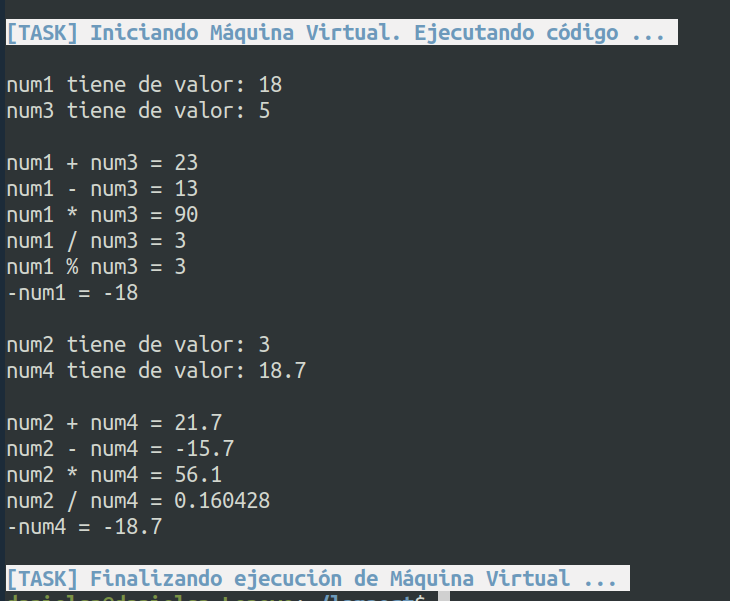
\includegraphics[width=\linewidth]{images/ejemplos/arithmeticOperations.png}
    \caption{Ejecución de programa: operaciones aritméticas.}
    \label{fig:lamportArithmeticOperations_exec}
\end{figure}

\newpage
\subsection{Ejemplo 2: Operaciones lógicas}
\begin{lstlisting}[style=lamportStyle]
{Programa: logical_operations.lmp}
{Autor: Daniel Perez Ruiz}

program Operaciones;
	var a : boolean := true;
	var b : boolean := false;

process Main;
	var c : boolean := true;
begin
	print("a es: ",a);
	print("b es: ",b);
	print("c es: ",c);
	print("");
	
	print("a y b es: ",a and b);
	print("a y c es: ",a and c);
	print("a y b y c es: ",a and b and c);
	print("");
	
	print("a o b es: ",a or b);
	print("a o c es: ",a or c);
	print("a o b o c es: ",a or b or c);
	print("");
	
	print("(a o b) y c es: ", (a or b) and c);
	print("(a o c) y b es: ", (a or c) and b);
	print("");
	
	print("no a es: ",not a);
	print("no b es: ",not b);
	
end
\end{lstlisting}
\begin{figure}[h]
\caption{Programa Lamport: operaciones lógicas}
\label{fig:lamportLogicalOperations}
\end{figure}

\newpage
\begin{figure}[h]
    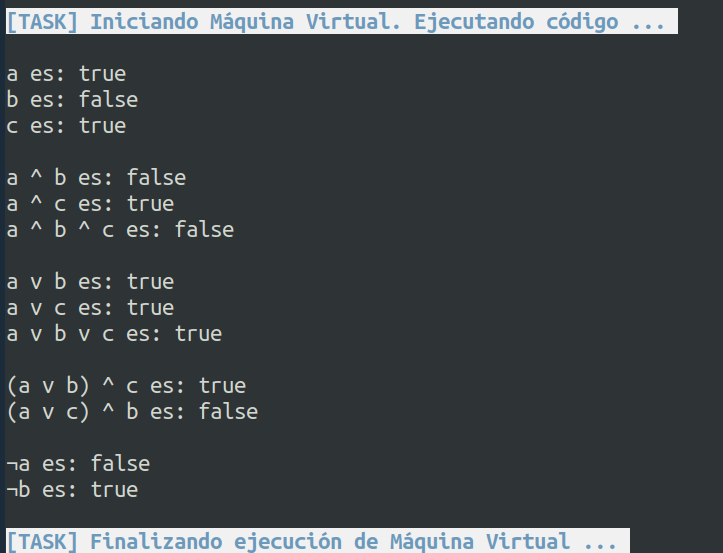
\includegraphics[width=\linewidth]{images/ejemplos/logical_operations.png}
    \caption{Ejecución de programa: operaciones lógicas.}
    \label{fig:lamportLogicalOperations_exec}
\end{figure}

\newpage
\subsection{Ejemplo 3: If/Else}
\begin{lstlisting}[style=lamportStyle]
{Programa: ifelse.lmp}
{Autor: Daniel Perez Ruiz}

program CompruebaEdad;
	var nombre1 : string := "Jorge";
	var edad1 : integer := 17;
	
	var nombre2 : string := "Pablo";
	var edad2 : integer := 22;
	
process main;
	var minimaEdad : integer := 18;
begin
	print(nombre1, ", tu edad es: ",edad1,". Comprobando si puedes entrar...");
	
	if edad1 < minimaEdad then
		begin
			print("NO puedes entrar. Debes tener ",minimaEdad," para poder entrar.");
		end
	else
		begin
			print("Adelante!!. Puedes entrar");
		end
		
	print("");
		
	print(nombre2, ", tu edad es: ",edad2,". Comprobando si puedes entrar...");
	
	if edad2 < minimaEdad then
		begin
			print("NO puedes entrar. Debes tener ",minimaEdad," para poder entrar.");
		end
	else
		begin
			print("Adelante!!. Puedes entrar");
		end
end
\end{lstlisting}
\begin{figure}[h]
\caption{Programa Lamport: flujos de control if/else.}
\label{fig:lamportIfElse}
\end{figure}

\newpage
\begin{figure}[h]
    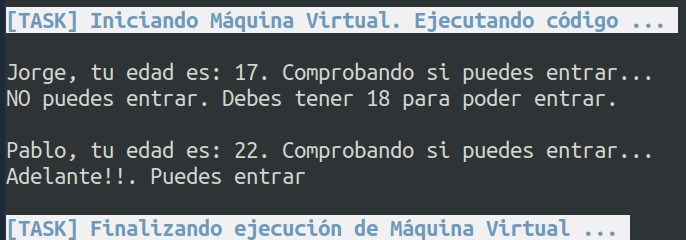
\includegraphics[width=\linewidth]{images/ejemplos/if_else.png}
    \caption{Ejecución de programa: if/else.}
    \label{fig:lamportIfElse_exec}
\end{figure}

\newpage
\subsection{Ejemplo 4: For}
\begin{lstlisting}[style=lamportStyle]
{Programa: for.lmp}
{Autor: Daniel Perez Ruiz}

program Bucles
	var contador : integer := 5;

process main;
	var startFor : integer := 1;
	var endFor : integer := 5;
begin
	print("La variable contador empieza en: ",contador);
	print("");
	print("Bucle for empieza en: ",startFor);
	print("Bucle for acaba en: ",endFor);
	
	print("");
	
	for i := startFor to endFor do
	begin
		contador := contador+1;
		print("--- contador vale ahora: ",contador);
		print("--- i vale: ", i);
	end
	
	print("");
	print("Ejecutando bucles anidados ...");
	print("");
	
	for j := 1 to 3 do
	begin
		print("------ j vale: ",j);
		for k := j to 4 do
		begin
			print("--- k vale: ",k);
		end
		print("");
	end
	
end
\end{lstlisting}
\begin{figure}[h]
\caption{Programa Lamport: bucles for.}
\label{fig:lamportFor}
\end{figure}

\newpage
\begin{figure}[!h]
    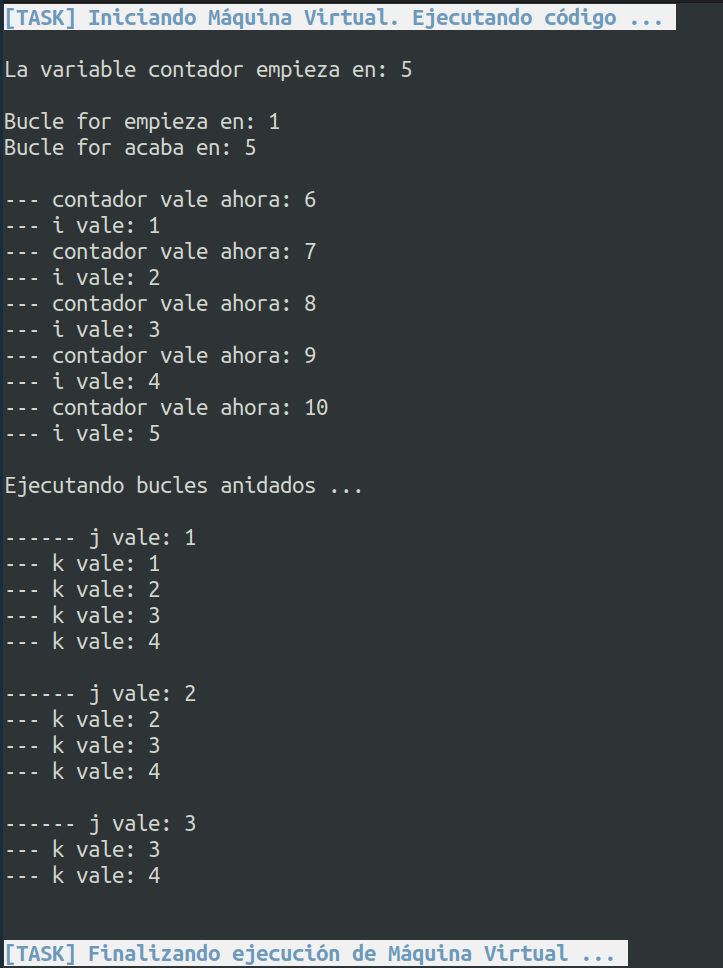
\includegraphics[scale=0.5]{images/ejemplos/for.png}
    \caption{Ejecución de programa: bucles for.}
    \label{fig:lamportFor_exec}
\end{figure}

\newpage
\subsection{Ejemplo 5: While}
\begin{lstlisting}[style=lamportStyle]
{Programa: while.lmp}
{Autor: Daniel Perez Ruiz}

program Bucles
	var contador : integer := 5;

process main;
	var valorMaximo : integer := 10;
begin
	print("La variable contador empieza en: ",contador);
	print("Su valor maximo debe ser: ",valorMaximo);
	print("");
	
	while contador < valorMaximo do
	begin
		contador := contador + 1;
		print(" --- Contador vale ahora: ", contador);
	end
	
	print(""); print("Fin de bucle");
end
\end{lstlisting}
\begin{figure}[h]
\caption{Programa Lamport: bucles while.}
\label{fig:lamportWhile}
\end{figure}

\newpage
\begin{figure}[h]
    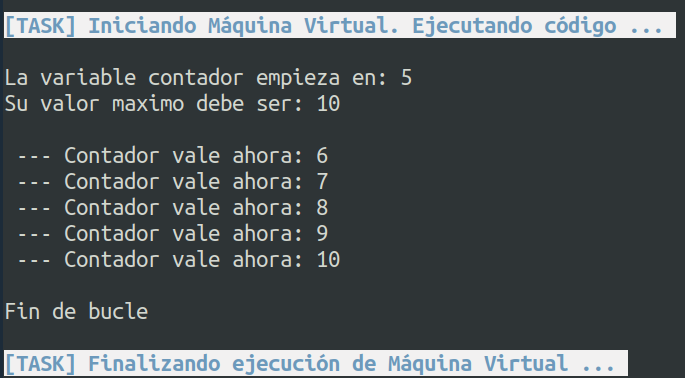
\includegraphics[width=\linewidth]{images/ejemplos/while.png}
    \caption{Ejecución de programa: bucles while.}
    \label{fig:lamportWhile_exec}
\end{figure}

\newpage
\subsection{Ejemplo 6: Uso de arrays}
\begin{lstlisting}[style=lamportStyle]
{Programa: for.lmp}
{Autor: Daniel Perez Ruiz}

program Arrays
	var numeros : array [5] integer;
process main;
	var letras : array [3] char;
begin
	print("Asignando numeros pares a array de numeros...");
	for i := 0 to 4 do
	begin
		print("Asignando a numeros[",i,"] el valor ",2*i);
		numeros[i] := 2*i;
	end
	
	print("");
	print("Imprimiendo array de numeros...");
	for j := 0 to 4 do
	begin
		print("numeros[",j,"] = ",numeros[j]);
	end
	
	letras[1] := 'd';
	print("");
	print("letras[1] es : ",letras[1]);
end
\end{lstlisting}
\begin{figure}[h]
\caption{Programa Lamport: uso de arrays}
\label{fig:lamportArray}
\end{figure}

\newpage
\begin{figure}[h]
    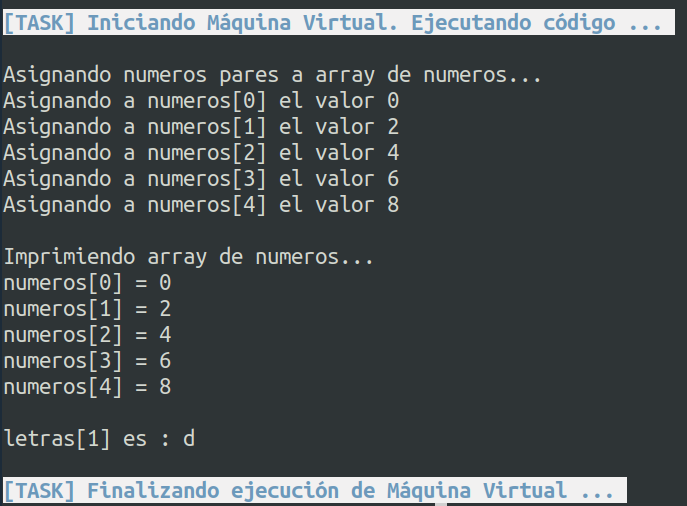
\includegraphics[width=\linewidth]{images/ejemplos/array.png}
    \caption{Ejecución de programa: arrays.}
    \label{fig:lamportArray_exec}
\end{figure}

\newpage
\section{Ejemplos que lanzan errores}
Los siguientes ejemplos mostrados son incorrectos, ya sean sintáctica o semánticamente, por lo que el intérprete lanzará los pertinentes mensajes de error.

\subsection{Ejemplo 1: Errores sintácticos en declaraciones}
\begin{lstlisting}[style=lamportStyle]
{Fichero: err_syntax_declarations.lmp}
{Autor: Daniel Perez Ruiz}
{Descripcion: Errores sintacticos de declaraciones}

program SyntaxErrors
	{CORRECTO}
	var v1 : integer;
	var v2 : string := "Hola";
	{ERROR}
	v3 : real;
	var 4v : boolean;
	var v5 char;
	var v6: string

process Main;
	{ERROR}
	var v7 : inventado;
	var v9 : array [5] invent;
	var v10 : integer := ;
	var v11 : integer 2+3;
	var v12 : integer := 1
begin
	print("Syntax errors!");
end
\end{lstlisting}
\begin{figure}[h]
\caption{Programa Lamport: errores sintácticos en declaraciones}
\label{fig:lamportErrSintaxDecl}
\end{figure}

\newpage
\begin{figure}[h]
    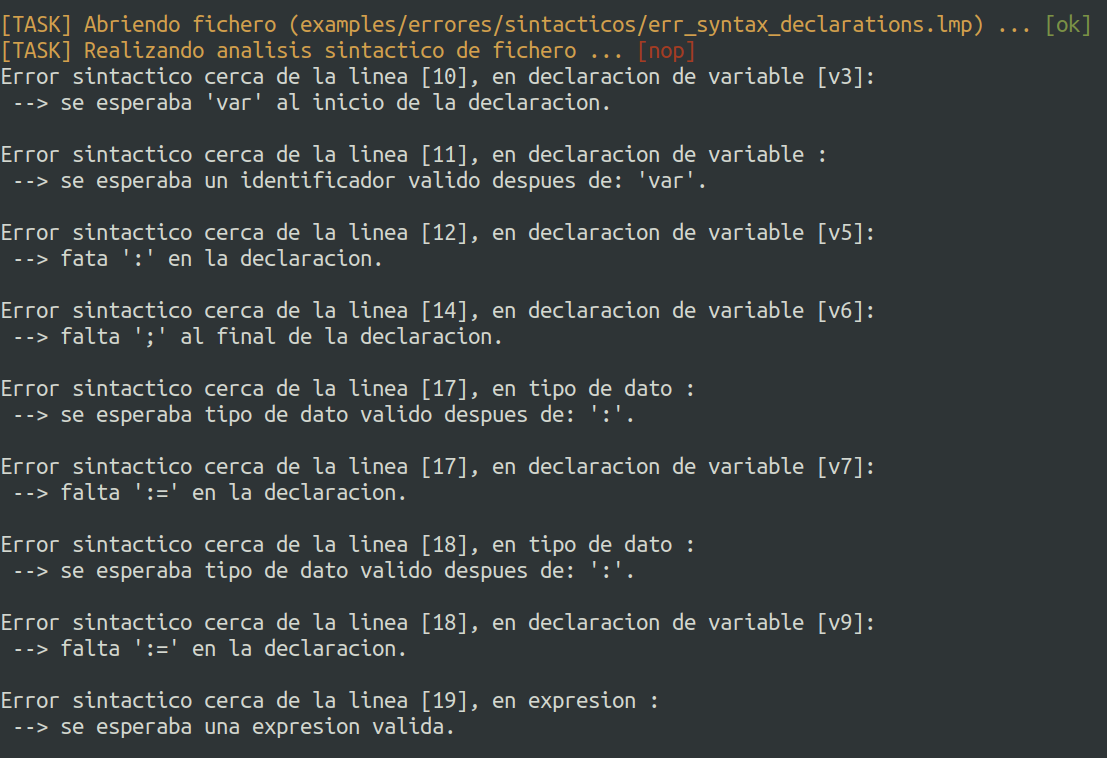
\includegraphics[width=\linewidth]{images/ejemplos/err_syntax/declarations.png}
    \caption{Ejecución de programa: errores sintácticos en declaraciones.}
    \label{fig:lamportErrSintaxDecl_exec}
\end{figure}

\newpage
\subsection{Ejemplo 2: Errores sintácticos en procedimientos}
\begin{lstlisting}[style=lamportStyle]
{Fichero: err_syntax_procedure.lmp}
{Autor: Daniel Perez Ruiz}
{Descripcion: Errores sintacticos de procedimientos}

program SyntaxErrors

{CORRECTO}
procedure imprimeEdad(a : string, b : integer);
begin
	print("Hola ",a,", tu edad es: ",b);
end

{CORRECTO}
procedure saluda();
begin
	print("hola");
end

{ERROR}
procedure proc1()
begin
	print("proc1");
end

{ERROR}
procedure 2proc();
	var v2 : invent;
begin
	print("fallo");
end

{ERROR}
procedure proc3(a : integer)
begin
	print("valor: ",a);
end

{ERROR}
procedure proc4(2 : integer);
begin
	print("fallo");
end

{ERROR}
procedure proc5(a char);
begin
	print("fallo");
end

{ERROR}
procedure proc6(a : invent);
begin
	print("fallo");
end

{ERROR}
procedure proc7(a : integer, b : invent);
begin
	print("fallo");
end

{ERROR}
procedure proc8(a : char,);
begin
	print("fallo");
end

process Main;
	{ERROR}
	var v1 : invent;
begin
	print("Syntax Errors!");
end
\end{lstlisting}
\begin{figure}[h]
\caption{Programa Lamport: errores sintácticos en procedimientos}
\label{fig:lamportErrSintaxProcedure}
\end{figure}

\newpage
\begin{figure}[h]
    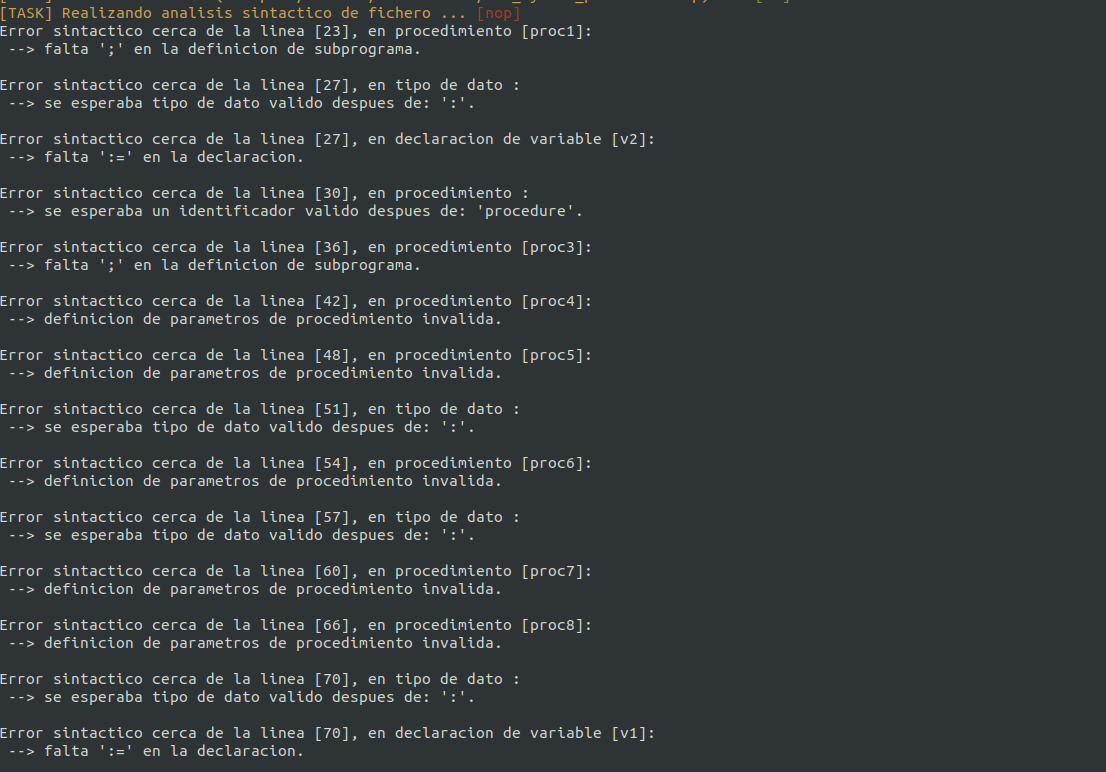
\includegraphics[width=\linewidth]{images/ejemplos/err_syntax/procedures.png}
    \caption{Ejecución de programa: errores sintácticos en procedimientos.}
    \label{fig:lamportErrSintaxProcedure_exec}
\end{figure}

\newpage
\subsection{Ejemplo 3: Errores semánticos: uso de variable no definida}
\begin{lstlisting}[style=lamportStyle]
{Fichero: undef_variable.lmp}
{Autor: Daniel Perez Ruiz}
{Descripcion: Contiene un error semantico de tipo: uso de variables no definidas}

program OperaEnteros

function suma(a: integer, b: integer) : integer;
begin
	{ERROR: Uso de variable no definida: resultadoSuma}
	resultadoSuma := a+b;
	return resultadoSuma;
end

procedure resta(a: integer, b: integer);
	var resultado : integer;
begin
	{ERROR: Uso de variable no definida: c}
	resultado := a - c;
	print(resultado);
end

process Main;
begin
	{ERROR: Uso de variable no definida: resultado}
	resultado := suma(3,5);
	{ERROR: Uso de variable no definida: num2}
	resta(3,num2);
end
\end{lstlisting}
\begin{figure}[h]
\caption{Programa Lamport: errores semánticos de no definición de variables.}
\label{fig:lamportErrSemanticUndef}
\end{figure}

\newpage
\begin{figure}[h]
    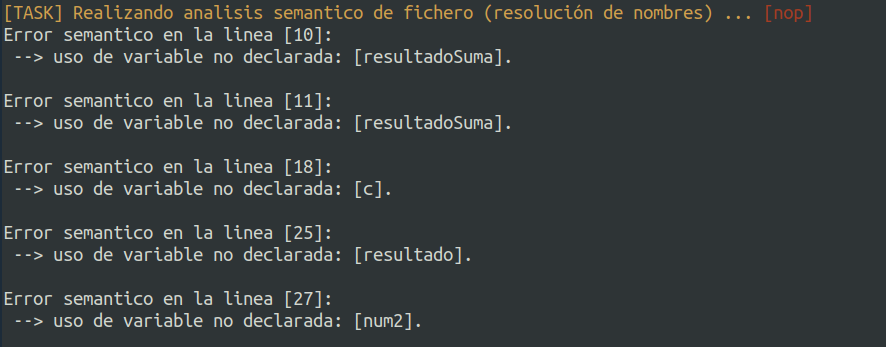
\includegraphics[width=\linewidth]{images/ejemplos/err_semantic/undef.png}
    \caption{Ejecución de programa: errores semánticos de no definición de variables.}
    \label{fig:lamportErrSemanticUndef_exec}
\end{figure}

\newpage
\subsection{Ejemplo 4: Errores semánticos: redefinición de variable}
\begin{lstlisting}[style=lamportStyle]
{Fichero: redef_variable.lmp}
{Autor: Daniel Perez Ruiz}
{Descripcion: Contiene un error semantico de tipo: redefinicion de variable}

program SumaEnteros
	var v1 : integer := 0;
	{ERROR: Redefinicion de variable}
	var v1 : integer;

process Main;
	var resultado : integer := 0;
	{ERROR: Redefinicion de variable}
	var resultado : char;
	{CORRECTO: este v1 esta en otro scope}
	var v1 : string := "hola";
begin
	{Invoca a la funcion para obtener el resultado}
	resultado := v1 + 2;
end
\end{lstlisting}
\begin{figure}[h]
\caption{Programa Lamport: errores semánticos de redefinición de variables.}
\label{fig:lamportErrSemanticRedef}
\end{figure}

\begin{figure}[h]
    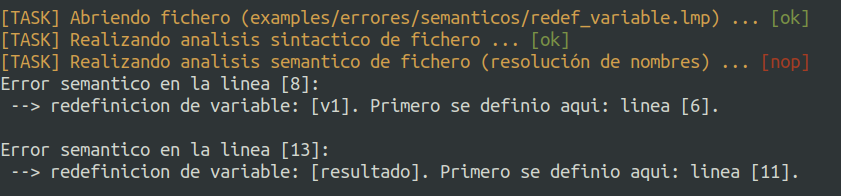
\includegraphics[width=\linewidth]{images/ejemplos/err_semantic/redef.png}
    \caption{Ejecución de programa: errores semánticos de no definición de variables.}
    \label{fig:lamportErrSemanticRedef_exec}
\end{figure}

\newpage
\subsection{Ejemplo 5: Errores semánticos: comprobación de tipos}
\begin{lstlisting}[style=lamportStyle]
{Fichero: typecheck_expressions.lmp}
{Autor: Daniel Perez Ruiz}
{Descripcion: Contiene errores semanticos de typechecking: expresiones}

program Sentencias
	var v1 : boolean := false;
	var v2 : string;
	var v3 : integer;
	
process Main;
	var v4 : real := 8.5;
	var resultado1 : integer;
	var resultado2 : real;
begin
	resultado1 := 1 + 3 * v3 - 1;
	{ERROR}
	resultado2 := v3 + 1.0 - 3;
	{ERROR}
	resultado1 := 1.0 - 10 / 2 + 7.5;
	{ERROR}
	resultado2 := 1 + 5 * 4;
	{ERROR}
	resultado2 := v2 + 3 / 2.5 - 1;
end
\end{lstlisting}
\begin{figure}[h]
\caption{Programa Lamport: errores semánticos en comprobación de tipos (expresiones).}
\label{fig:lamportErrSemanticTypecheck}
\end{figure}

\newpage
\begin{figure}[h]
    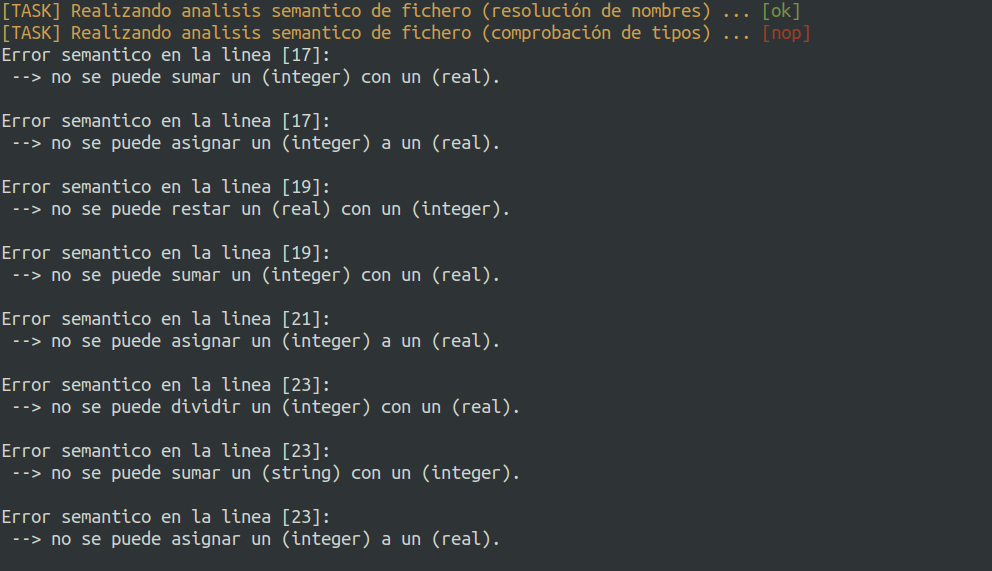
\includegraphics[width=\linewidth]{images/ejemplos/err_semantic/typecheck.png}
    \caption{Ejecución de programa: errores semánticos en comprobación de tipos (expresiones).}
    \label{fig:lamportErrSemanticTypecheck_exec}
\end{figure}

\newpage
\section{Ejemplos que lanzan excepciones}
Los siguientes ejemplos mostrados son correctos sintácticamente y semánticamente. Sin embargo, realizan operaciones no permitidas, y generan una excepción en la Máquina Virtual.

\subsection{Ejemplo 1: Excepción ZeroDivision}
\begin{lstlisting}[style=lamportStyle]
{Programa: zerodivision.lmp}
{Autor: Daniel Perez Ruiz}

program Operaciones
	var num1 : integer := 1;

process Main;
	var num2 : integer := 0;
	var resultado : integer;
begin
	{GENERA EXCEPCION EN LVM: Division zero}
	resultado := num1/num2;
end
\end{lstlisting}
\begin{figure}[h]
\caption{Programa Lamport: excepción ZeroDivision}
\label{fig:lamportExceptionZeroDivision}
\end{figure}

\begin{figure}[h]
    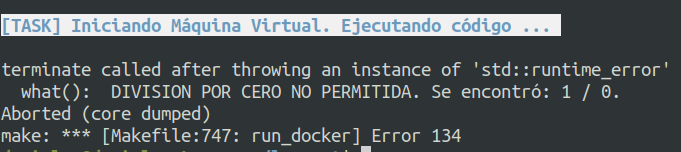
\includegraphics[width=\linewidth]{images/ejemplos/exceptions/zerodivision.png}
    \caption{Ejecución de programa: excepción ZeroDivision.}
    \label{fig:lamportExceptionZeroDivision_exec}
\end{figure}

\newpage
\subsection{Ejemplo 2: Excepción IndexOutOfBounds}
\begin{lstlisting}[style=lamportStyle]
{Programa: out_of_bounds.lmp}
{Autor: Daniel Perez Ruiz}

program Arrays
	var numeros : array [5] integer;

procedure negativeBound();
begin
	{EXCEPCION: Se intenta acceder a una posicion negativa de array}
	numeros[-2] := 2;
end

procedure excedBound();
begin
	{EXCEPCION: Se intenta acceder a una posicion negativa de array}
	numeros[6] := -2;
end

procedure printBadArray();
begin
	for i := 0 to 5 do
	begin
		print(numeros[i]);
	end
end
	
{INTERCAMBIE EL ORDEN DE EJECUCION PARA VER LAS EXCEPCIONES}
process main;
begin
	{EXCEPCION TIPO 2: Acceso a region fuera del limite superior}
	excedBound();
	
	{EXCEPCION TIPO 3: Recorrido en bucle que se sale de los limites}
	printBadArray();

	{EXCEPCION TIPO 1: Acceso negativo}
	negativeBound();
end
\end{lstlisting}
\begin{figure}[h]
\caption{Programa Lamport: excepción IndexOutOfBounds.}
\label{fig:lamportExceptionOutOfBounds}
\end{figure}

\newpage
\begin{figure}[h]
    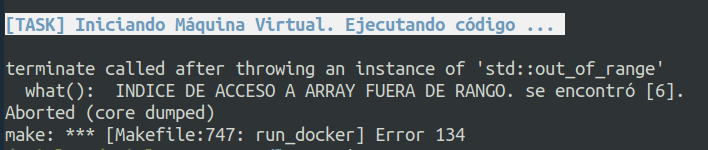
\includegraphics[width=\linewidth]{images/ejemplos/exceptions/out_of_bounds.png}
    \caption{Ejecución de programa: excepción IndexOutOfBounds.}
    \label{fig:lamportExceptionOutOfBounds_exec}
\end{figure}

\section{Ejemplos concurrentes}
Para finalizar, ha llegado el momento de verificar si se ha solucionado el problema que se planteó en el capítulo ~\ref{chapter:problema}, que es el de \textit{disponer de un lenguaje que permita simular sistemas concurrentes}. A continuación, se presenta una serie de ejemplos detallados que requiere de uso de concurrencia en el intérprete:

\subsection{Ejemplo 1: Múltiples procesos estáticos}
En este ejemplo se dispone de 3 procesos estáticos cuyo propósito es imprimir un mensaje por pantalla que consta de dos elementos: un mensaje de saludo seguido de una variable entera que actúa a modo de identificador de proceso. Estos mensajes están dentro de un bucle infinito, por lo que cada proceso se ejecutará indefinidamente:
\begin{lstlisting}[style=lamportStyle]
{Programa: race_condition.lmp}
{Autor: Daniel Perez Ruiz}

program Race

process P1;
	var id : integer := 1;
begin
	while true do
	begin
		print("te saluda el proceso: ",id);
	end
end

process P2;
	var id : integer := 2;
begin
	while true do
	begin
		print("te saluda el proceso: ",id);
	end
end

process P3;
	var id : integer := 3;
begin
	while true do
	begin
		print("te saluda el proceso: ",id);
	end
end
\end{lstlisting}
\begin{figure}[h]
\caption{Programa Lamport: múltiples procesos estáticos (race condition)}
\label{fig:lamportMultipleProcess}
\end{figure}

\begin{figure}[h]
    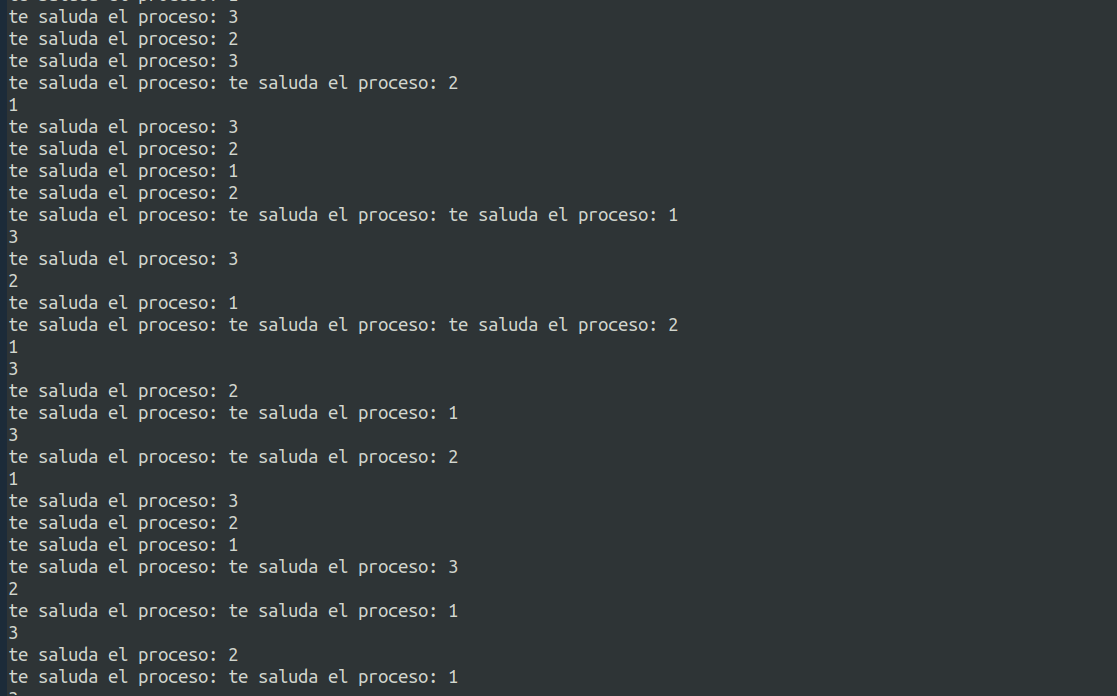
\includegraphics[width=\linewidth]{images/ejemplos/concurrentes/multiple_process.png}
    \caption{Ejecución de programa: múltiples procesos estáticos (race condition).}
    \label{fig:lamportMultipleProcess_exec}
\end{figure}

Se puede apreciar que efectivamente los tres procesos muestran mensajes. Sin embargo, en algunas ocasiones no se muestran correctamente porque se entrelazan las instrucciones de impresión de unos procesos con otros.

\newpage

\subsection{Ejemplo 2: Múltiples procesos estáticos (con sección atómica)}
Para solucionar el problema anterior, se puede introducir un bloque de secciones atómicas que contengan a las instrucciones de impresión en cada proceso, como se muestra a continuación:
\begin{lstlisting}[style=lamportStyle]
{Programa: atomic.lmp}
{Autor: Daniel Perez Ruiz}

program NotARace

process P1;
	var id : integer := 1;
begin
	while true do
	begin
		<< print("te saluda el proceso: ",id); >>
	end
end

process P2;
	var id : integer := 2;
begin
	while true do
	begin
		<< print("te saluda el proceso: ",id); >>
	end
end

process P3;
	var id : integer := 3;
begin
	while true do
	begin
		<< print("te saluda el proceso: ",id); >>
	end
end
\end{lstlisting}
\begin{figure}[h]
\caption{Programa Lamport: múltiples procesos estáticos (con sección atómica)}
\label{fig:lamportMultipleProcessAtomic}
\end{figure}

\newpage
\begin{figure}[h]
    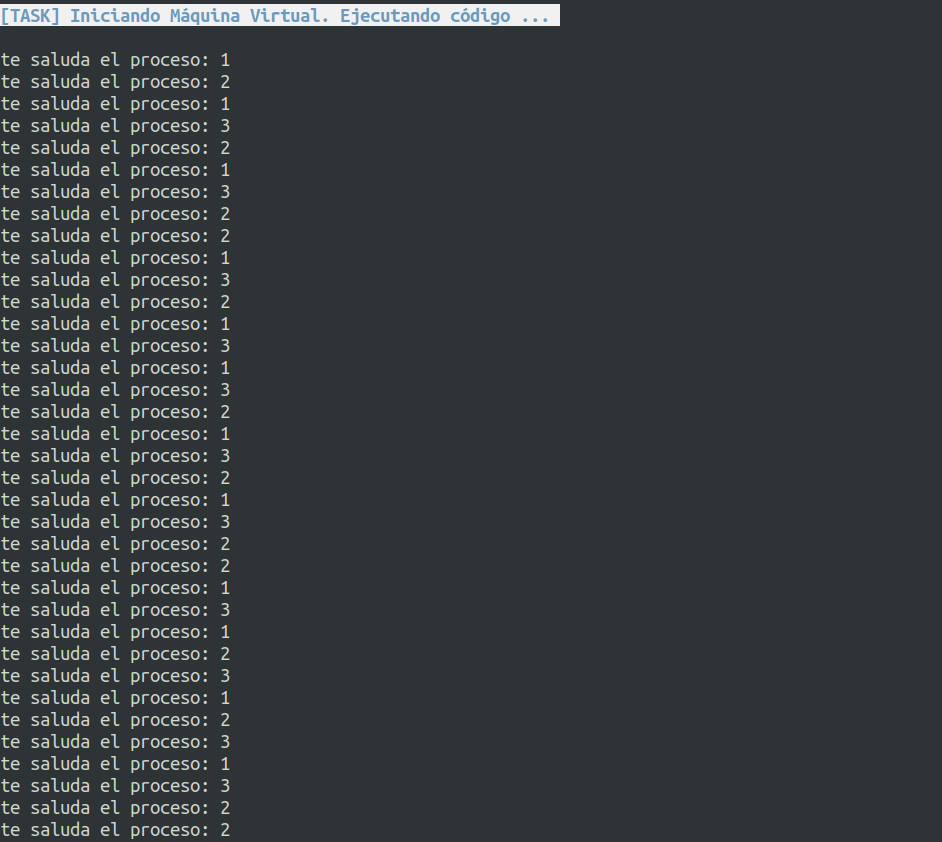
\includegraphics[width=\linewidth]{images/ejemplos/concurrentes/multiple_process_atomic.png}
    \caption{Ejecución de programa: múltiples procesos estáticos (con sección atómica)}
    \label{fig:lamportMultipleProcessAtomic_exec}
\end{figure}

Ahora, los tres procesos también muestran mensajes, pero se muestran ordenadamente debido a que, cuando una hebra entra en una sección atómica, se ejecutan todas las instrucciones que contiene hasta que termina. En este caso, se ejecutan 3 instrucciones dentro de cada sección atómica: saludo, índice y salto de línea.

\newpage
\subsection{Ejemplo 3: Vector de procesos estáticos}
En este ejemplo también se dispone de 3 procesos, pero han sido definidos mediante un vector indexado. Cada proceso dispone de su propio valor de índice, y lo utilizará para incrementar una variable compartida a los 3 procesos denominada \code{total}. El valor esperado final de la variable total es 6.
\begin{lstlisting}[style=lamportStyle]
{Programa: process_vector.lmp}
{Autor: Daniel Perez Ruiz}

program SumaIndice

	var total : integer := 0;

process VectorProc[index: 1..3];
begin
    total := total + index;
   	print("proceso (",index,") incrementa total a: ", total);
end
\end{lstlisting}
\begin{figure}[h]
\caption{Programa Lamport: vector de procesos estáticos (race condition).}
\label{fig:lamportProcessVector}
\end{figure}

\begin{figure}[h]
    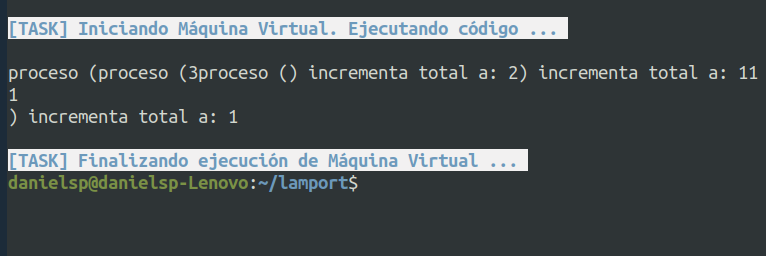
\includegraphics[width=\linewidth]{images/ejemplos/concurrentes/vector_process.png}
    \caption{Ejecución de programa: vector de procesos estáticos (race condition).}
    \label{fig:lamportProcessVector_exec}
\end{figure}

El resultado de esta ejecución es un caos tremendo debido a la concurrencia. No sólo en cuanto al contenido de los mensajes sino también en el resultado final que debería tener la variable global \code{total}.

\newpage
\subsection{Ejemplo 4: Vector de procesos estáticos (con atomic)}
Nuevamente, para solucionar el problema del ejemplo anterior es suficiente con definir una sección atómica que englobe a las dos instrucciones de los procesos.
\begin{lstlisting}[style=lamportStyle]
{Programa: process_vector_atomic.lmp}
{Autor: Daniel Perez Ruiz}

program SumaIndice

	var total : integer := 0;

process VectorProc[index: 1..3];
begin
    << total := total + index;
   	print("proceso (",index,") incrementa total a: ", total); >>
end
\end{lstlisting}
\begin{figure}[h]
\caption{Programa Lamport: vector de procesos estáticos (atómico).}
\label{fig:lamportProcessVectorAtomic}
\end{figure}

\begin{figure}[h]
    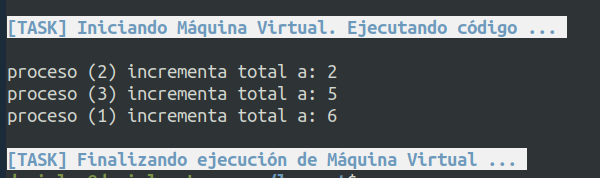
\includegraphics[width=\linewidth]{images/ejemplos/concurrentes/vector_process_atomic.png}
    \caption{Programa Lamport: vector de procesos estáticos (atómico).}
    \label{fig:lamportProcessVectorAtomic_exec}
\end{figure}

Aunque el orden de ejecución de los procesos puede ser diferente cada vez que se ejecute el programa, gracias a la sección atómica definida cada proceso muestra claramente el mensaje, y siempre el último mostrará que el resultado de la variable \code{total} es 6, como se esperaba.

\newpage
\subsection{Ejemplo 5: Bloque de instrucciones concurrentes (cobegin-coend)}
En el siguiente ejemplo se define una variable global denominada \code{x} cuyo valor inicial es 0. Después se define un proceso \code{Main} que contiene dos instrucciones de impresión y un bloque de instrucciones concurrentes. Puesto que al igual que en los otros ejemplos presentados aquí no se ha definido ningún mecanismo de sincronización, el resultado final de la variable \code{x} puede ser impredecible, aunque lo deseable sería que fuese 0.
\begin{lstlisting}[style=lamportStyle]
{Programa: cobegin.lmp}
{Autor: Daniel Perez Ruiz}

program Cobegin
	var x : integer := 0;
	
process Main;
begin
	print("iniciando bloque cobegin ...");

	cobegin
		x := x+1;
		x := x-1;
	coend
	
	print("x vale: ",x);
end
\end{lstlisting}
\begin{figure}[h]
\caption{Programa Lamport: bloque de instrucciones concurrentes cobegin-coend (race condition).}
\label{fig:lamportCobegin}
\end{figure}

\newpage

\begin{figure}[h]
    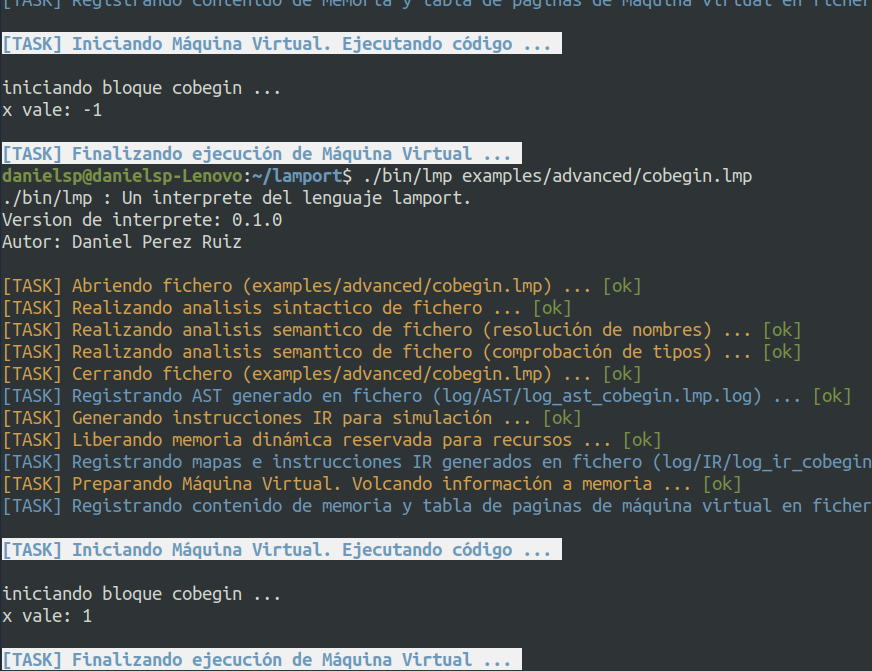
\includegraphics[width=\linewidth]{images/ejemplos/concurrentes/cobegin.png}
    \caption{Ejecución de programa: bloque de instrucciones concurrentes cobegin-coend (race condition).}
    \label{fig:lamportCobegin_exec}
\end{figure}

En estas dos ejecuciones del programa se ha obtenido un valor diferente: 1 y -1. De hecho, el conjunto de valores posibles para la variable \code{x} es: -1,0,1. Esto es evidentemente causado por el entrelazamiento de las hebras.

\vspace{0.5cm}
Notar además que, cuando se entra en un bloque cobegin, el proceso \code{Main} espera de manera implícita a que se ejecuten todas las hebras creadas dinámicamente para ejecutar todas las instrucciones que contiene.

\newpage
\subsection{Ejemplo 6: Bloque de instrucciones concurrentes (cobegin-coend) (con atomic)}
Si incluimos cada instrucción del bloque cobegin-coend en un bloque atómico, se soluciona el problema anteriormente mencionado.
\begin{lstlisting}[style=lamportStyle]
{Programa: cobegin.lmp}
{Autor: Daniel Perez Ruiz}

program Cobegin
	var x : integer := 0;
	
process Main;
begin
	print("iniciando bloque cobegin ...");

	cobegin
		<< x := x+1; >>
		<< x := x-1; >>
	coend
	
	print("x vale: ",x);
end
\end{lstlisting}
\begin{figure}[h]
\caption{Programa Lamport: bloque de instrucciones concurrentes cobegin-coend (atómico).}
\label{fig:lamportCobeginAtomic}
\end{figure}

\newpage

\begin{figure}[h]
    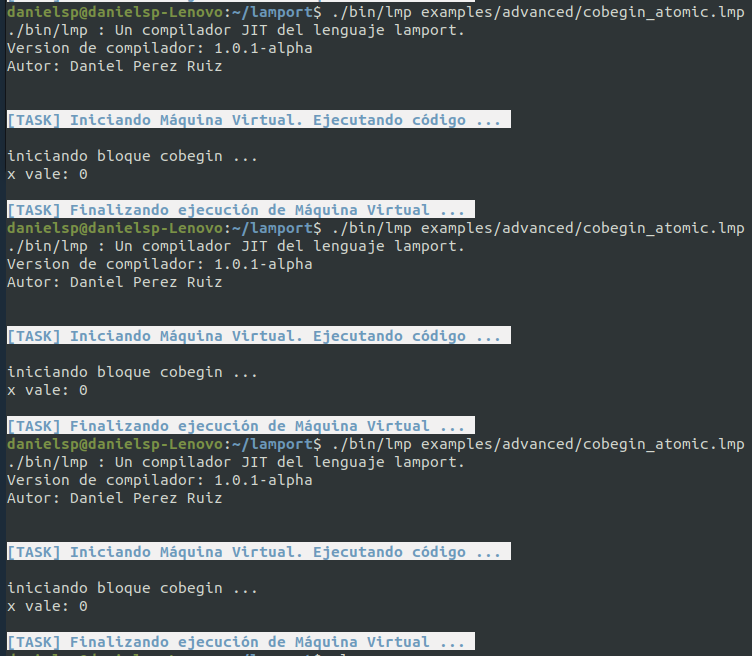
\includegraphics[width=\linewidth]{images/ejemplos/concurrentes/cobegin_atomic.png}
    \caption{Ejecución de programa: bloque de instrucciones concurrentes cobegin-coend (atómico).}
    \label{fig:lamportCobeginAtomic_exec}
\end{figure}

Ahora siempre que se ejecute este programa el resultado obtenido será 0, verificando así la buena sincronización de las hebras dentro de un bloque de instrucciones concurrentes de este tipo.

\newpage
\subsection{Ejemplo 7: Ejecución y sincronización de procedimientos concurrentes con fork-join}
En este ejemplo disponemos de una variable global \code{x} y dos procedimientos que hacen dos tareas diferentes. Uno incrementa la variable \code{x} unas 100 veces, y otro lo decrementa unas 20 veces. El resultado final que debería tener la variable es \code{x = 80}. Ejecutándolo secuencialmente, se verifica sin problema, pero el objetivo de este programa es ejecutar sendos procedimientos concurrentemente. 

\vspace{0.5cm}

El proceso \code{Main} indica a Increment que se ejecute concurrentemente con la llamada que realiza después a decrement, utilizando la sentencia \code{fork}. Con la sentencia \code{join}, la hebra \code{Main} se bloquea esperando a que \code{Increment()} termine su ejecución.
\begin{lstlisting}[style=lamportStyle]
{Programa: fork_join.lmp}
{Autor: Daniel Perez Ruiz}

program Fork;
	var x : integer := 0;

procedure Increment();
begin
	for i := 1 to 100 do
	begin
		x := x+1;
	end
	
	print("fin de increment");
end

procedure Decrement();
begin
	for j := 1 to 20 do
	begin
		x := x-1;
	end
	
	print("fin de decrement");
end

process Main;
begin
	print("Realizando fork...");
	fork Increment;
	Decrement();
	join;
	
	print("x vale: ",x);
	
	
	if(x == 80) then
	begin
		print("Se ha obtenido 80, el valor esperado");
	end
	else
	begin
		print("No se ha obtenido 80.");
	end
end
\end{lstlisting}
\begin{figure}[h]
\caption{Programa Lamport: creación y sincronización de hebras dinámicas con fork-join.}
\label{fig:lamportForkJoin}
\end{figure}

\newpage

\begin{figure}[h]
    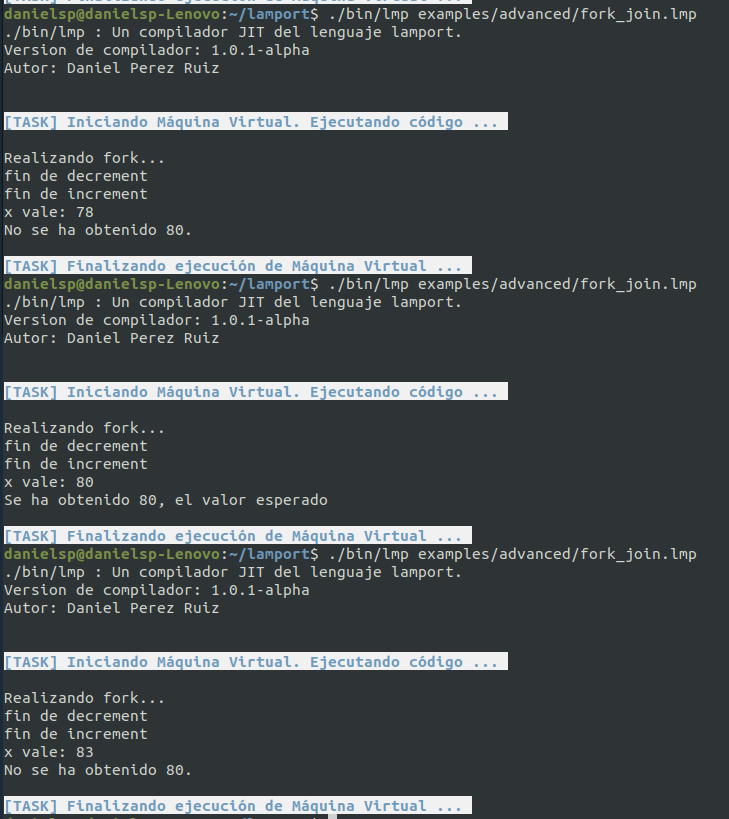
\includegraphics[width=\linewidth]{images/ejemplos/concurrentes/fork_join.png}
    \caption{Ejecución de programa: creación y sincronización de hebras dinámicas con fork-join.}
    \label{fig:lamportForkJoin_exec}
\end{figure}

Se observa que la sincronización de Increment con la hebra principal Main se realiza adecuadamente, pues los mensajes que se escribieron después de join se ejecutan sí y sólo sí cuando este procedimiento ha terminado. Sin embargo, se vuelve a apreciar que en dos ejecuciones del programa no hay el resultado esperado, obteniendo dos resultados diferentes.

\newpage
Si las instrucciones de las líneas 11 y 21 se engloban dentro de una sección atómica, el resultado de la ejecución del programa es el siguiente, donde siempre se conseguirá el valor deseado de la variable \code{x}.

\begin{figure}[h]
    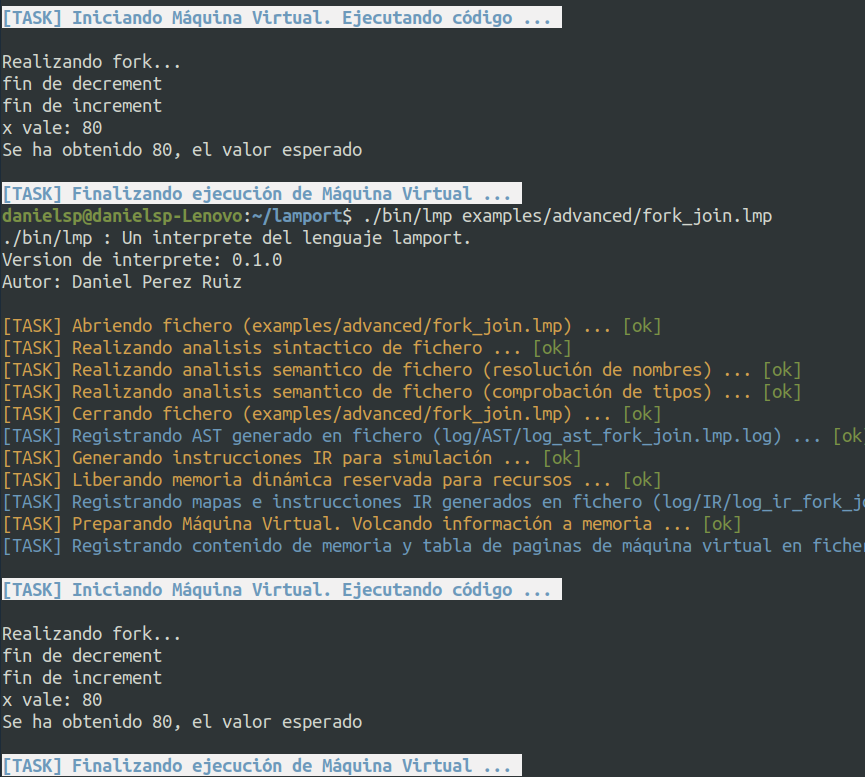
\includegraphics[width=\linewidth]{images/ejemplos/concurrentes/fork_join_atomic.png}
    \caption{Ejecución de programa: creación y sincronización de hebras dinámicas con fork-join (atómico).}
    \label{fig:lamportForkJoinAtomic_exec}
\end{figure}

\newpage
Finalmente, queda preguntarse qué sucede si se elimina la instrucción \code{join} (línea 32) que es quien sincroniza al proceso \code{Main} con su hija. Lo más probable es que lo que ocurra sea que la hebra principal termine antes que su hija, un comportamiento poco deseado y que se aprecia a continuación:

\begin{figure}[h]
    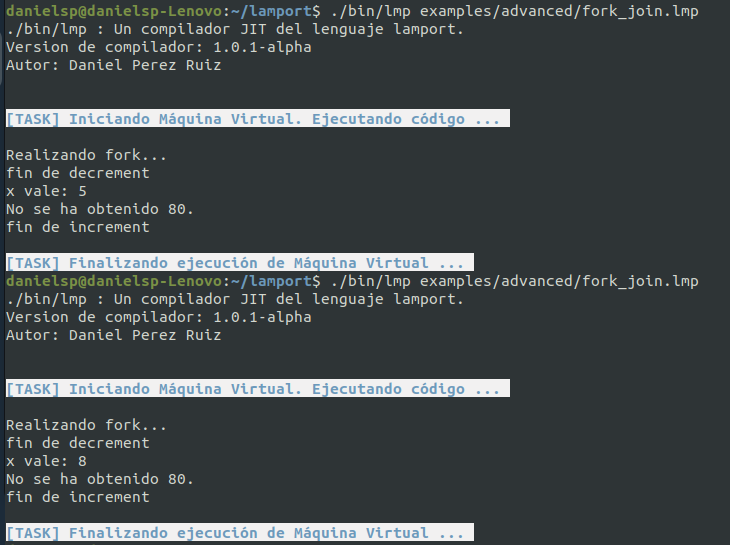
\includegraphics[width=\linewidth]{images/ejemplos/concurrentes/fork_without_join.png}
    \caption{Ejecución de programa: creación y sincronización de hebras dinámicas con fork (sin join).}
    \label{fig:lamportForkWithoutJoin_exec}
\end{figure}

Se observa que los mensajes de impresión después de la llamada a los procedimientos se muestran antes de que Increment notifique que ha terminado.

\newpage
\subsection{Ejemplo 8: Sincronización de procedimientos concurrentes con semáforos}
Este ejemplo es bastante parecido al anterior, con la salvedad de que se tiene otra forma diferente de sincronizar los procedimientos \code{Increment} y \code{Decrement}. Se observa un semáforo denominado \code{sem} y cuyo valor de inicio es 1.

\vspace{0.5cm}

Un semáforo es una herramienta de sincronización utilizada en la programación concurrente para controlar el acceso a un recurso compartido. Funciona como un contador, y sus operaciones fundamentales son \code{WAIT} (o también llamada \textit{P}) y \code{SIGNAL} (o \textit{V}). El \code{WAIT} disminuye el contador y, si este es negativo, bloquea el proceso; mientras que el \code{SIGNAL} incrementa el contador y, si hay procesos bloqueados, permite que uno de ellos continue su ejecución. De esta manera, los semáforos pueden garantizar que ciertas secciones de código no sean ejecutadas por más de un proceso a la vez, evitando condiciones de carrera y otros problemas relacionados con la concurrencia.

\begin{lstlisting}[style=lamportStyle]
{Programa: semaphore.lmp}
{Autor: Daniel Perez Ruiz}
program Semaphore;
    var x : integer := 2;
    var sem : semaphore := 1;

procedure Increment();
begin
    for i := 1 to 5 do
    begin
        WAIT sem;
        print("Incrementando x, que vale ahora: ", x);
        x := x + 1;
        SIGNAL sem;
    end
end

procedure Decrement();
begin
    for i := 1 to 5 do
    begin
        WAIT sem;
        print("Decrementando x, que vale ahora: ", x);
        x := x - 1;
        SIGNAL sem;
    end
end

process Main;
begin
    fork Increment;
    fork Decrement;
    join;
    print("x vale: ", x);
end
\end{lstlisting}
\begin{figure}[h]
\caption{Programa Lamport: sincronización de procesos con semáforo.}
\label{fig:lamportSemaphore}
\end{figure}

\begin{figure}[h]
    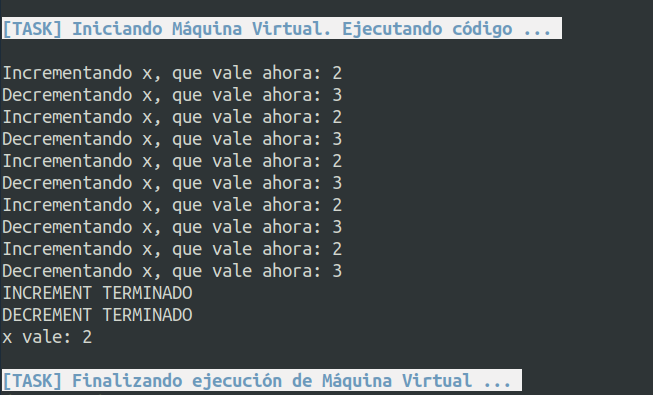
\includegraphics[width=\linewidth]{images/ejemplos/concurrentes/semaphore.png}
    \caption{Ejecución de programa: sincronización de procesos con semáforo.}
    \label{fig:lamportSemaphore_exec}
\end{figure}

En esta ejecución se observa que cada procedimiento modifica una única vez el valor de la variable global, dando como resultado final 2, que era el valor esperado tras incrementar y decrementar 1 unidad el número, el mismo número de veces.